\documentclass[12pt,letterpaper]{article}
\usepackage[margin=1in]{geometry}
\usepackage{chngpage}
\usepackage[english]{babel}
\usepackage[utf8x]{inputenc}
\usepackage{amsmath}
\usepackage{amssymb} 
% \usepackage[retainorgcmds]{IEEEtrantools}
\usepackage{graphicx}
\usepackage{tabularx}
\usepackage{kpfonts}    % for nice fonts
\usepackage{microtype} 
\usepackage{booktabs}   % for nice tables
\usepackage{bm}         % for bold math
\usepackage{listings}   % for inserting code
\usepackage{verbatim}   % useful for program listings
\usepackage{color}  
\usepackage[colorlinks=true]{hyperref}
% use for hypertext
\hypersetup{
	colorlinks=false,       % false: boxed links; true: colored links
	linkcolor=green,        % color of internal links
	citecolor=blue,        % color of links to bibliography
	filecolor=magenta,     % color of file links
	urlcolor=blue         
}
\usepackage[colorinlistoftodos]{todonotes}
\usepackage{natbib}
\usepackage{float}
\usepackage{adjustbox}
\usepackage[capitalise]{cleveref}
\usepackage{xcolor}

\usepackage{longtable,threeparttablex}
\usepackage{subcaption}



%++++++++++++++++++++++++++++++++++++++++


\begin{document}

\begin{center}
\large IEMS-469 Dynamic Programming  HW1

\bigskip
Weijia Zhao \footnote{Weijia.Zhao@kellogg.northwestern.edu}\\
Kellogg Finance

\bigskip
This version: \today
\end{center}

\newpage

\section{Single Class Problem}
The order of events at time t is: dispatch of a shuttle $\rightarrow$ new consumers come $\rightarrow$ calculate waiting cost.  \footnote{One can easily modify the code to reflect a different assumption under which new consumers can be picked by immediately by the shuttle. This is even more straightforward given that I use s\_remaining and s\_remaining\_new to represent the number of consumers waiting in the line after the shuttle pick up and after the new consumers come. In the end the results do not change much for these two assumptions except that the value function under primary assumption equals to the value function under alternative assumption minus a constant, as all consumers need to wait at least one period under the primary assumption}\\

I use pretty strict converging criteria in all the exercise, the maximal iteration possible is $10^7$ (for value iteration, the outer loop and inner loop of policy iteration) and the error tolerance is $10^{-6}$ (again, for value iteration, the outer loop and inner loop of policy iteration).\\

I finished the homework assignment before this week's lecture and I use V for both the value function with only state as its argument ("V" in reinforcement learning) and the value function with both state and action as its argument ("Q" in reinforcement learning) following Econ/Fin tradition. \\

The initial value function or initial policy function in any of the three methods can be initialized randomly\footnote{Enumeration method requires V to be all 0 as the the residual value after the last period should be 0 but in this example, T is so large that it will converge after 500 iterations so that doesn't really matter. So the enumeration method is actually identical to value iteration method except the counters/termination requirement of iteration are different}. I initialize the value function to be all 0 and policy function to be all 0. \\

The usage of V(s) and Q(s,a) can be interchangeable as these two functions as closely related to each other. In enumeration and value iteration methods, $V(s)=max_{a} Q(s,a)$. In policy iteration, actions are given by policy $\pi$. Then we only fill the only policy cells when construct $Q(s,a)$, leave all the off policy cells blank, and only focus on those none blank cells, we get back to $V(s)$.\\

All the graphs follow my expectation, we have a cut-off strategy, dispatch a shuttle if and only if the number of people waiting is above a certain threshold. The value function is a decreasing function of the number of people waiting. 
\begin{figure}[H]
	\centering
	\caption{Single Class Problem}
	\begin{subfigure}[h]{0.48\textwidth}
		\centering
		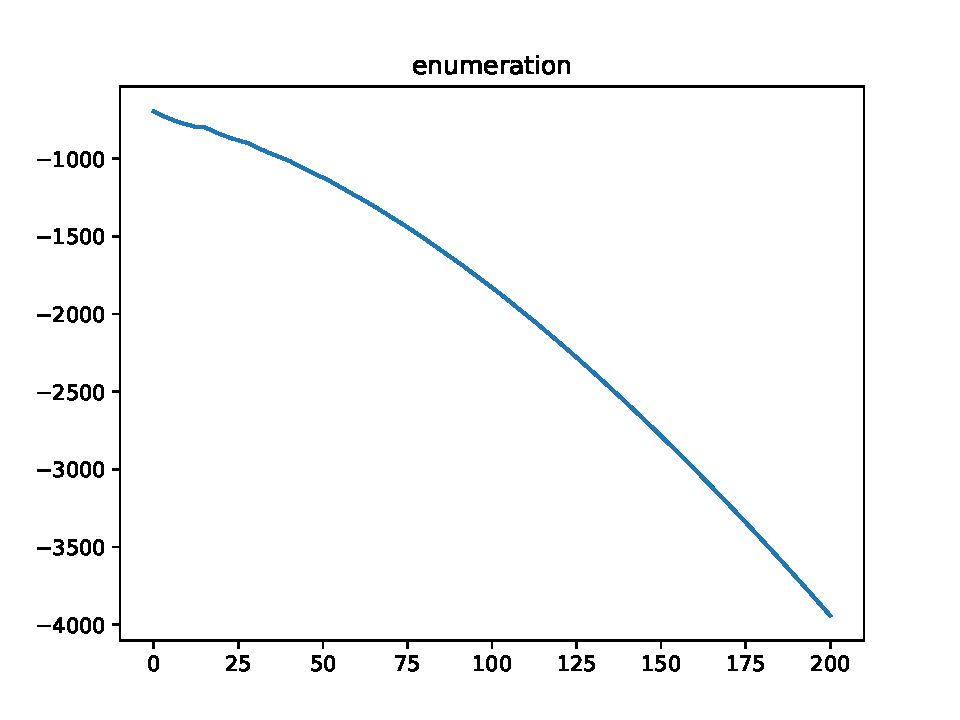
\includegraphics[width=\textwidth]{/Users/lesliezhao/Dropbox/nu_course/2021_fall/DP/IEMS469_HW_LWZ/hw1/q1_enumeration.pdf}
		\caption{Enumeration: Value Function}
	\end{subfigure}
	\begin{subfigure}[h]{0.48\textwidth}
		\centering
		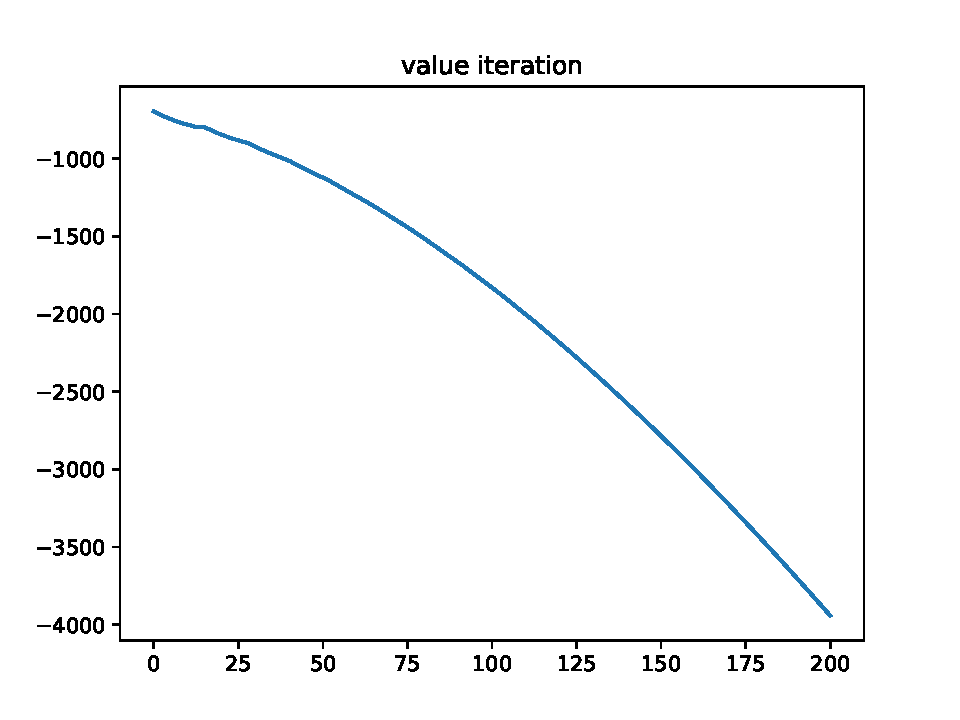
\includegraphics[width=\textwidth]{/Users/lesliezhao/Dropbox/nu_course/2021_fall/DP/IEMS469_HW_LWZ/hw1/q1_value_iteration.pdf}
		\caption{Value Iteration: Value Function}
	\end{subfigure}
	\begin{subfigure}[h]{0.48\textwidth}
		\centering
		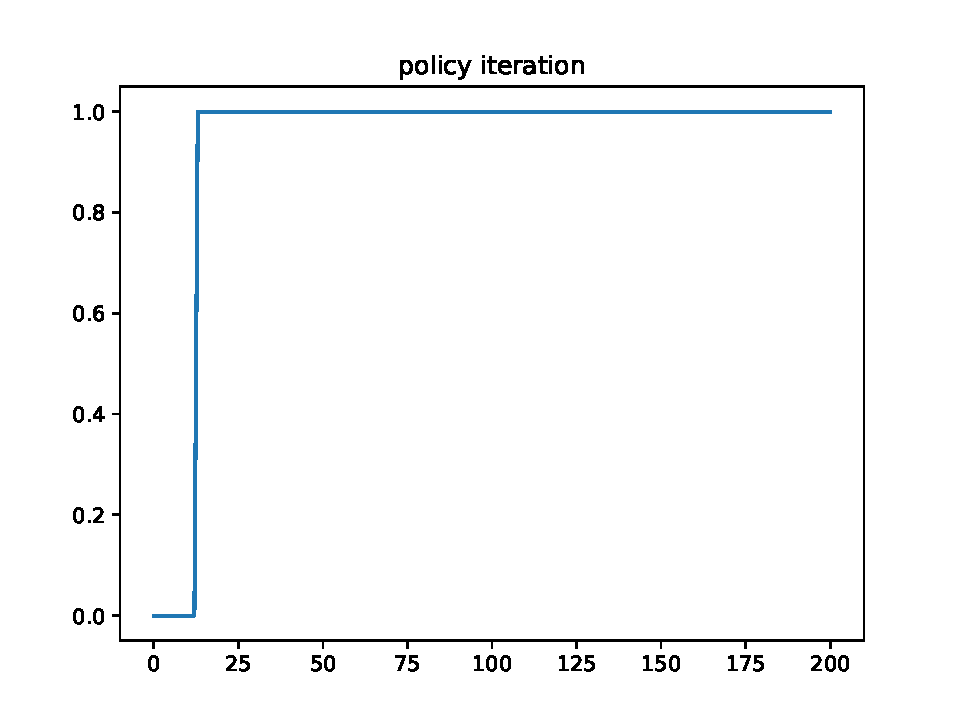
\includegraphics[width=\textwidth]{/Users/lesliezhao/Dropbox/nu_course/2021_fall/DP/IEMS469_HW_LWZ/hw1/q1_policy_iteration.pdf}
		\caption{Policy Iteration: Policy Function}
	\end{subfigure}
	\label{votemap}
\end{figure}

\section{Multi Class Problem}
Apparently with the parameters suggested by the homework assignment, the state space is $100*100*100*100*100=10000000000=10^{10}$ and the transition matrix contains $10^{20}$ elements. This type of curse of dimensionality prevents us from getting any meaningful results in  reasonable time period. Instead, I reduce the state space by looking at individuals with waiting time $\{2,2.5,3\}$ and the limit of each type is 30\footnote{Parameters suggested in the homework are listed in commented area}. I get the following results, where states are indexed by (num1,num2,num3) where numi is the number of people waiting in the line that are of ith type. \footnote{The states are first sorted by num1 then num2 then num3. That is the reason why the density of policy function taking value 0 decrease because at the beginning, num1 is small and we allow num2 and num3 to be slightly larger but as num1 getting larger the threshold for num2 and num3 also decrease.} \\

I also tried to use the parameters given in Q1 to verify the correctness of my code and it turns out they generate exactly the same results.
\begin{figure}[H] 
	\centering
	\caption{Option Characteristics}
	\begin{subfigure}[h]{0.48\textwidth}
		\centering
		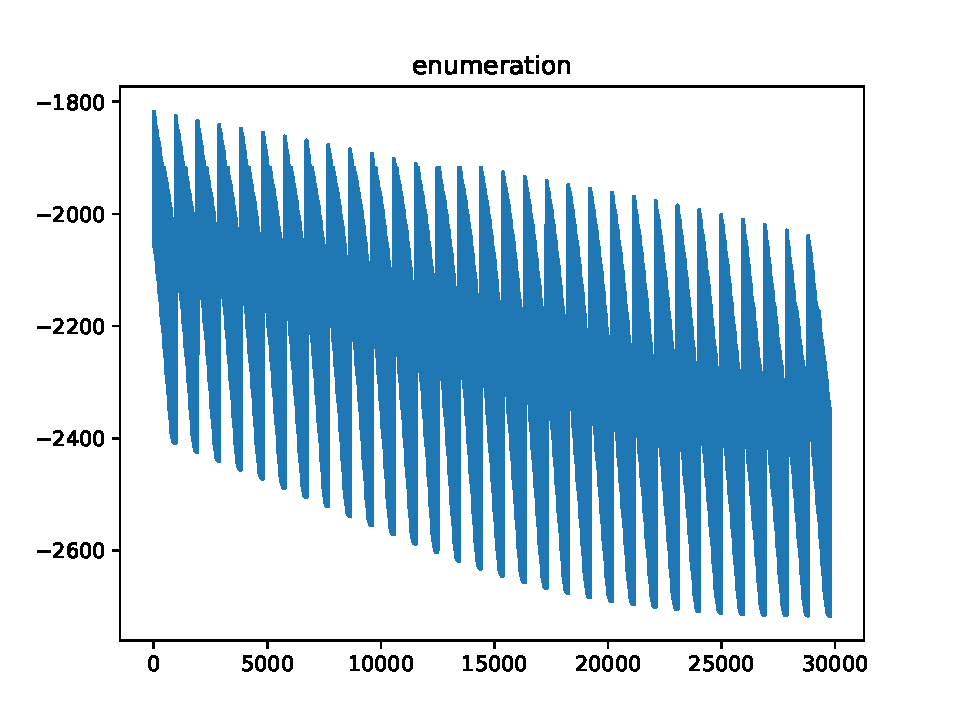
\includegraphics[width=\textwidth]{/Users/lesliezhao/Dropbox/nu_course/2021_fall/DP/IEMS469_HW_LWZ/hw1/q2_enumeration.pdf}
		\caption{GDP in year 2016}
	\end{subfigure}
	\begin{subfigure}[h]{0.48\textwidth}
		\centering
		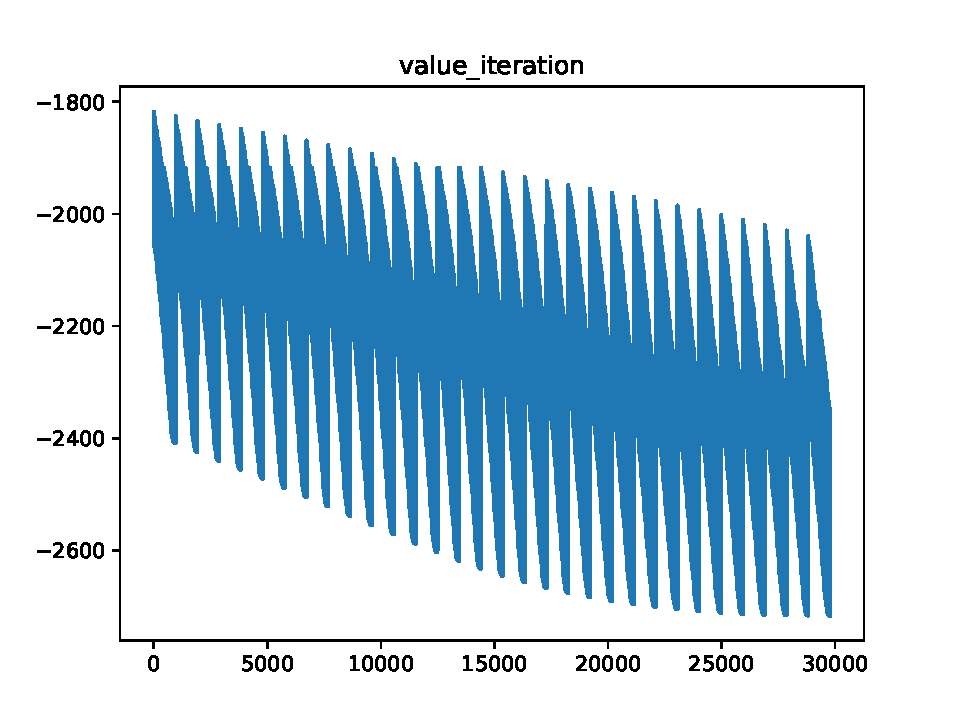
\includegraphics[width=\textwidth]{/Users/lesliezhao/Dropbox/nu_course/2021_fall/DP/IEMS469_HW_LWZ/hw1/q2_value_iteration.pdf}
		\caption{Bond value matched}
	\end{subfigure}
	\begin{subfigure}[h]{0.48\textwidth}
		\centering
		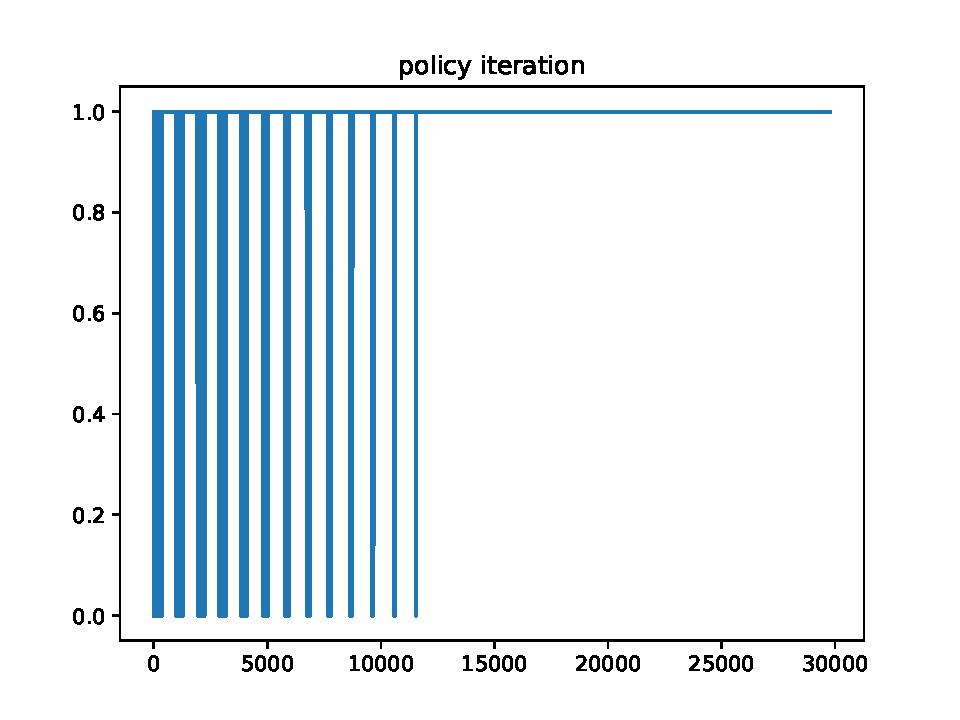
\includegraphics[width=\textwidth]{/Users/lesliezhao/Dropbox/nu_course/2021_fall/DP/IEMS469_HW_LWZ/hw1/q2_policy_iteration.pdf}
		\caption{GDP in year 2016}
	\end{subfigure}
	\label{votemap}
\end{figure}
\clearpage
\setlength



\end{document}
